% LaTeX document skeleton
% generated on Tue Jan 04 15:00:38 +0100 2011
% by Kévin Fardel et Rick Ghanem
% With the Condom lib (version 1.1.0)
% See http://github.com/v0n/condom

%%%%%%%%%%%%%
% PREAMBULE %
%%%%%%%%%%%%%

\documentclass[a4paper, 11pt]{article}           % format general

% LaTeX packages to import
% generated on Tue Jan 04 15:00:38 +0100 2011
% by Kévin Fardel et Rick Ghanem
% With the Condom lib (version 1.1.0)
% See http://github.com/v0n/condom

\usepackage[T1]{fontenc}      % codage des caracteres

\usepackage[utf8]{inputenc}   % encodage du fichier (utf8 ou latin1)
\usepackage[francais]{babel}  % langue
\usepackage{mathpazo}         % selection de la police
\usepackage{geometry}         % mise en page
\usepackage{xcolor}           % pour colorer des elements

\usepackage{graphicx}         % pour inserer des images

% math
\usepackage{amssymb}          % symboles mathematiques
%\usepackage{amsmath}         % commandes mathematiques

% pdf
\usepackage{url}              % permet l'insertion d'url
\usepackage[pdftex]{hyperref} % permet l'hypertexte (rend les liens cliquables)

% listings
\usepackage{listings}         % permet d'inserer du code (multi-langage)
\usepackage{courier}
\usepackage{caption}

% fancyhdr
\usepackage{lastpage}         % derniere page
\usepackage{fancyhdr}         % en-tete et pied de page

\usepackage{multicol}


\input{inc/colors}
% Personal commands
% generated on Tue Jan 04 15:00:38 +0100 2011
% by Kévin Fardel et Rick Ghanem
% With the Condom lib (version 1.1.0)
% See http://github.com/v0n/condom

% raccourcis
\newcommand{\Cad}{C'est-à-dire~}
\newcommand{\cad}{c'est-à-dire~}
\newcommand{\pe}{peut-être~}

\newcommand{\todo}[1]{\bigskip \colorbox{myyellow}{\textcolor{mygrey}{\textsf{\textbf{TODO} #1 }}} \bigskip}

\newcommand{\name}[2]{#1 \textsc{#2}}

\newcommand{\email}[1]{\href{mailto:#1}{\textsf{<#1>}}}

% commande pour afficher un lien vers une image
\newcommand{\figref}[1]{\textsc{Fig.}~\ref{#1} (p.~\pageref{#1})}

% commande pour afficher le lien vers un listing :
\newcommand{\lstref}[1]{{\footnotesize Listing~\ref{#1}, p.~\pageref{#1}}}



% listings package config file
% generated on Tue Jan 04 15:00:38 +0100 2011
% by Kévin Fardel et Rick Ghanem
% With the Condom lib (version 1.1.0)
% See http://github.com/v0n/condom

% /!\ ne pas utiliser de caracteres accentues dans les sources (ne gere pas l'utf-8)
% pour remplacer les lettres accentues : sed -i -e "y/ÉÈÊÇÀÔéèçàôîêûùï/EEECAOeecaoieuui/" fichier

% configuration des listings par defaut :
\lstset{ %
	language={},                % choose the language of the code
	basicstyle=\footnotesize,       % the size of the fonts that are used for the code
	numbers=left,                   % where to put the line-numbers
	numberstyle=\footnotesize,      % the size of the fonts that are used for the line-numbers
	stepnumber=2,                   % the step between two line-numbers. If it's 1 each line 
	numbersep=5pt,                  % how far the line-numbers are from the code
	backgroundcolor=\color{white},  % choose the background color. You must add \usepackage{color}
	showspaces=false,               % show spaces adding particular underscores
	showstringspaces=false,         % underline spaces within strings
	showtabs=false,                 % show tabs within strings adding particular underscores
	frame=single,	                % adds a frame around the code
	tabsize=2,	                % sets default tabsize to 2 spaces
	captionpos=b,                   % sets the caption-position to bottom
	breaklines=true,                % sets automatic line breaking
	breakatwhitespace=false,        % sets if automatic breaks should only happen at whitespace
	title=\lstname,                 % show the filename of files included with \lstinputlisting;
	commentstyle=\color{blue},                                % also try caption instead of title
	keywordstyle=\color{green},
    	ndkeywordstyle=\color{darkgreen},
    	identifierstyle=\color{cyan},
    	stringstyle=\color{red},
	escapeinside={\%*}{*)},         % if you want to add a comment within your code
	morekeywords={*,...}            % if you want to add more keywords to the set
}

\lstloadlanguages{
    %[Visual]Basic
    %Pascal
    %C
    %C++
    %XML
    %HTML
    %Java
}
%\DeclareCaptionFont{blue}{\color{blue}}

%\captionsetup[lstlisting]{singlelinecheck=false, labelfont={blue}, textfont={blue}}
\DeclareCaptionFont{white}{\color{white}}
\DeclareCaptionFormat{listing}{\colorbox[cmyk]{0.43, 0.35, 0.35,0.01}{\parbox{\textwidth}{\hspace{15pt}#1#2#3}}}
\captionsetup[lstlisting]{format=listing,labelfont=white,textfont=white, singlelinecheck=false, margin=0pt, font={bf,footnotesize}}

% configuration des listings console :
\lstnewenvironment{console}
{\lstset{%
    language={},
    numbers=none,
    extendedchars=true,
    framexleftmargin=5mm,
    %float,
    showstringspaces=false,
    showspaces=false,
    showtabs=false,
    breaklines=false,
    backgroundcolor=\color{darkgray},
    basicstyle=\color{white} \scriptsize \ttfamily,
    keywordstyle=\color{white},
    ndkeywordstyle=\color{white},
    commentstyle=\color{white},
    identifierstyle=\color{white},
    stringstyle=\color{white}
}}
{}

\renewcommand{\lstlistlistingname}{Table des codes sources} % renommer la liste des listings

% un listing depuis un fichier s'importe comme ceci :
%\lstinputlisting[caption={Legende}, label=lst:label]{emplacement}

                        % fichier de config du paquet listings

\geometry{top=2.5cm, bottom=2.5cm, left=2cm, right=2cm}

\graphicspath{{fig/}}                 % chemins vers les images

% informations du document
\author{Kévin Fardel et Rick Ghanem}
\date{\today}
\title{Rapport de Traitement du signal}

\hypersetup{%
    pdftitle    = {Rapport de Traitement du signal},
    pdfauthor   = {Kévin Fardel et Rick Ghanem}
    pdfcreator  = {Texlive},
    pdfproducer = {Texlive},
    colorlinks  = true,
    linkcolor   = black,
    citecolor   = black,
    urlcolor    = black
}                                                   % informations du pdf

\pagestyle{fancy}
\lhead{Rapport de Traitement du signal}
\chead{}
\rhead{\thepage/\pageref{LastPage}}
\lfoot{}
\cfoot{}
\rfoot{\footnotesize Kévin Fardel et Rick Ghanem}
%\renewcommand{\headrulewidth}{0pt}
%\renewcommand{\footrulewidth}{0.4pt}
\fancypagestyle{plain}{%                        % style des pages de titres
    \fancyhf{}
    \renewcommand{\headrulewidth}{0pt}
    \renewcommand{\footrulewidth}{0pt}
}

\makeatletter
\@addtoreset{section}{part} % reprendre a partir de 1 les sections des parties suivantes
\makeatother

%\AtBeginDocument{%
%   \renewcommand{\abstractname}{} % renommer le resume
%}

%%%%%%%%%
% CORPS %
%%%%%%%%%

\begin{document} % debut du document

\maketitle % afficher le titre

% resume
\begin{abstract}
\end{abstract}

\tableofcontents % table des matieres

\lstlistoflistings % tables des listings

\newpage
\part{Exercice 1}
\lstinputlisting[caption={Code source pour l'exercice 1}, label=lst:label, language=Octave]{src/ex1.m}

\part{Exercice 2}
\lstinputlisting[caption={Code source pour l'exercice 2}, label=lst:label, language=Octave]{src/ex2.m}

\lstinputlisting[caption={Fonction pour créer un echelon}, label=lst:label, language=Octave]{src/echelon.m}

\part{Exercice 3}
\section{Fonction $\frac{1-z^{-1}}{2}$}
Nous commençons par afficher le diagramme de gain en décibel (\ref{f1 Diagramme de gain}) ainsi que le diagramme de phase en radians (\ref{f1 Diagramme de phase}) pour déterminer la nature du filtre représenté par cette fonction de transfert.
\begin{figure}[H]
\centering
\includegraphics[width=9cm]{resEx3/f1Gain.pdf}
\caption{Diagramme de gain de la fonction $\frac{1-z^{-1}}{2}$ en dB}
\label{f1 Diagramme de gain}
\end{figure}
\begin{figure}[H]
\centering
\includegraphics[width=9cm]{resEx3/f1Phase.pdf}
\caption{Diagramme de phase de la fonction $\frac{1-z^{-1}}{2}$ en radians}
\label{f1 Diagramme de phase}
\end{figure}
Nous pouvons donc constater que cette fonction de transfert en z correspond à un filtre passe haut.
\subsection{Réponse impulsionnelle}
~\\
\begin{figure}[H]
\centering
\includegraphics[width=9cm]{resEx3/f1Impulsion.pdf}
\caption{Réponse impulsionnelle de la fonction $\frac{1-z^{-1}}{2}$ }
\end{figure}
\subsection{Réponse indicielle}
~\\
\begin{figure}[H]
\centering
\includegraphics[width=9cm]{resEx3/f1Indice.pdf}
\caption{Réponse indicielle de la fonction $\frac{1-z^{-1}}{2}$ }
\end{figure}

\subsection{Les zéros et les pôles}
~\\
\begin{figure}[H]
\centering
\includegraphics[width=9cm]{resEx3/f1ZP.pdf}
\caption{Les zéros et les pôles de la fonction $\frac{1-z^{-1}}{2}$ }
\end{figure}


\section{Fonction $\frac{1+z^{-1}}{2}$}
Nous commençons par afficher le diagramme de gain en décibel (\ref{f2 Diagramme de gain}) ainsi que le diagramme de phase en radians (\ref{f2 Diagramme de phase}) pour déterminer la nature du filtre représenté par cette fonction de transfert.
\begin{figure}[H]
\centering
\includegraphics[width=9cm]{resEx3/f2Gain.pdf}
\caption{Diagramme de gain de la fonction $\frac{1+z^{-1}}{2}$ en dB}
\label{f2 Diagramme de gain}
\end{figure}
\begin{figure}[H]
\centering
\includegraphics[width=9cm]{resEx3/f2Phase.pdf}
\caption{Diagramme de phase de la fonction $\frac{1+z^{-1}}{2}$ en radians}
\label{f2 Diagramme de phase}
\end{figure}
Nous pouvons donc constater que cette fonction de transfert en z correspond à un filtre passe bas.
\subsection{Réponse impulsionnelle}
~\\
\begin{figure}[H]
\centering
\includegraphics[width=9cm]{resEx3/f2Impulsion.pdf}
\caption{Réponse impulsionnelle de la fonction $\frac{1+z^{-1}}{2}$ }
\end{figure}

\subsection{Réponse indicielle}
~\\
\begin{figure}[H]
\centering
\includegraphics[width=9cm]{resEx3/f2Indice.pdf}
\caption{Réponse indicielle de la fonction $\frac{1+z^{-1}}{2}$ }
\end{figure}

\subsection{Les zéros et les pôles}
~\\
\begin{figure}[H]
\centering
\includegraphics[width=9cm]{resEx3/f2ZP.pdf}
\caption{Les zéros et les pôles de la fonction $\frac{1+z^{-1}}{2}$ }
\end{figure}


\section{Fonction $\frac{1-z^{-2}}{2}$}
Nous commençons par afficher le diagramme de gain en décibel (\ref{f3 Diagramme de gain}) ainsi que le diagramme de phase en radians (\ref{f3 Diagramme de phase}) pour déterminer la nature du filtre représenté par cette fonction de transfert.
\begin{figure}[H]
\centering
\includegraphics[width=9cm]{resEx3/f3Gain.pdf}
\caption{Diagramme de gain de la fonction $\frac{1-z^{-2}}{2}$ en dB}
\label{f3 Diagramme de gain}
\end{figure}
\begin{figure}[H]
\centering
\includegraphics[width=9cm]{resEx3/f3Phase.pdf}
\caption{Diagramme de phase de la fonction $\frac{1-z^{-2}}{2}$ en radians}
\label{f3 Diagramme de phase}
\end{figure}
Nous pouvons donc constater que cette fonction de transfert en z correspond à un filtre passe bande.
\subsection{Réponse impulsionnelle}
~\\
\begin{figure}[H]
\centering
\includegraphics[width=9cm]{resEx3/f3Impulsion.pdf}
\caption{Réponse impulsionnelle de la fonction $\frac{1-z^{-2}}{2}$ }
\end{figure}

\subsection{Réponse indicielle}
~\\
\begin{figure}[H]
\centering
\includegraphics[width=9cm]{resEx3/f3Indice.pdf}
\caption{Réponse indicielle de la fonction $\frac{1-z^{-2}}{2}$ }
\end{figure}

\subsection{Les zéros et les pôles}
~\\
\begin{figure}[H]
\centering
\includegraphics[width=9cm]{resEx3/f3ZP.pdf}
\caption{Les zéros et les pôles de la fonction $\frac{1-z^{-2}}{2}$ }
\end{figure}


\section{Fonction $\frac{2z^{-1}}{2-z^{-1}}$}
Nous commençons par afficher le diagramme de gain en décibel (\ref{f4 Diagramme de gain}) ainsi que le diagramme de phase en radians (\ref{f4 Diagramme de phase}) pour déterminer la nature du filtre représenté par cette fonction de transfert.
\begin{figure}[H]
\centering
\includegraphics[width=9cm]{resEx3/f4Gain.pdf}
\caption{Diagramme de gain de la fonction $\frac{2z^{-1}}{2-z^{-1}}$ en dB}
\label{f4 Diagramme de gain}
\end{figure}
\begin{figure}[H]
\centering
\includegraphics[width=9cm]{resEx3/f4Phase.pdf}
\caption{Diagramme de phase de la fonction $\frac{2z^{-1}}{2-z^{-1}}$ en radians}
\label{f4 Diagramme de phase}
\end{figure}
Nous pouvons donc constater que cette fonction de transfert en z correspond à un filtre passe bas.
\subsection{Réponse impulsionnelle}
~\\
\begin{figure}[H]
\centering
\includegraphics[width=9cm]{resEx3/f4Impulsion.pdf}
\caption{Réponse impulsionnelle de la fonction $\frac{2z^{-1}}{2-z^{-1}}$}
\end{figure}

\subsection{Réponse indicielle}
~\\
\begin{figure}[H]
\centering
\includegraphics[width=9cm]{resEx3/f4Indice.pdf}
\caption{Réponse indicielle de la fonction $\frac{2z^{-1}}{2-z^{-1}}$}
\end{figure}

\subsection{Les zéros et les pôles}
~\\
\begin{figure}[H]
\centering
\includegraphics[width=9cm]{resEx3/f4ZP.pdf}
\caption{Les zéros et les pôles de la fonction $\frac{2z^{-1}}{2-z^{-1}}$ }
\end{figure}


\section{Fonction $\frac{2z^{-1}-z^{-5}}{2-z^{-1}}$}
Nous commençons par afficher le diagramme de gain en décibel (\ref{f5 Diagramme de gain}) ainsi que le diagramme de phase en radians (\ref{f5 Diagramme de phase}) pour déterminer la nature du filtre représenté par cette fonction de transfert.
\begin{figure}[H]
\centering
\includegraphics[width=9cm]{resEx3/f5Gain.pdf}
\caption{Diagramme de gain de la fonction $\frac{2z^{-1}-z^{-5}}{2-z^{-1}}$ en dB}
\label{f5 Diagramme de gain}
\end{figure}
\begin{figure}[H]
\centering
\includegraphics[width=9cm]{resEx3/f5Phase.pdf}
\caption{Diagramme de phase de la fonction $\frac{2z^{-1}-z^{-5}}{2-z^{-1}}$ en radians}
\label{f5 Diagramme de phase}
\end{figure}
Nous pouvons donc constater que cette fonction de transfert en z correspond à un filtre coupe bande.
\subsection{Réponse impulsionnelle}
~\\
\begin{figure}[H]
\centering
\includegraphics[width=9cm]{resEx3/f5Impulsion.pdf}
\caption{Réponse impulsionnelle de la fonction $\frac{2z^{-1}-z^{-5}}{2-z^{-1}}$ }
\end{figure}

\subsection{Réponse indicielle}
~\\
\begin{figure}[H]
\centering
\includegraphics[width=9cm]{resEx3/f5Indice.pdf}
\caption{Réponse indicielle de la fonction $\frac{2z^{-1}-z^{-5}}{2-z^{-1}}$ }
\end{figure}

\subsection{Les zéros et les pôles}
~\\
\begin{figure}[H]
\centering
\includegraphics[width=9cm]{resEx3/f5ZP.pdf}
\caption{Les zéros et les pôles de la fonction $\frac{2z^{-1}-z^{-5}}{2-z^{-1}}$ }
\end{figure}


\part{Exercice 4}
Nous créons un filtre passe bas de type Butterworth avec les caractéristiques suivantes:\\
\begin{itemize}
\item Fréquence d'échantillonnage : 8 kHz
\item Fréquence de coupure : 1 kHz
\item Largeur de transition : 200 Hz
\item Ondulation maximale dans la bande passante : 1 dB
\item Atténuation minimale dans la bande coupée : 40 dB
\end{itemize}
~\\
Les trois figures suivantes nous la réponse impulsionnelle, les pôles et les zéros ainsi que la fonction de transfert du filtre que nous avons créé.

\begin{figure}[H]
\centering
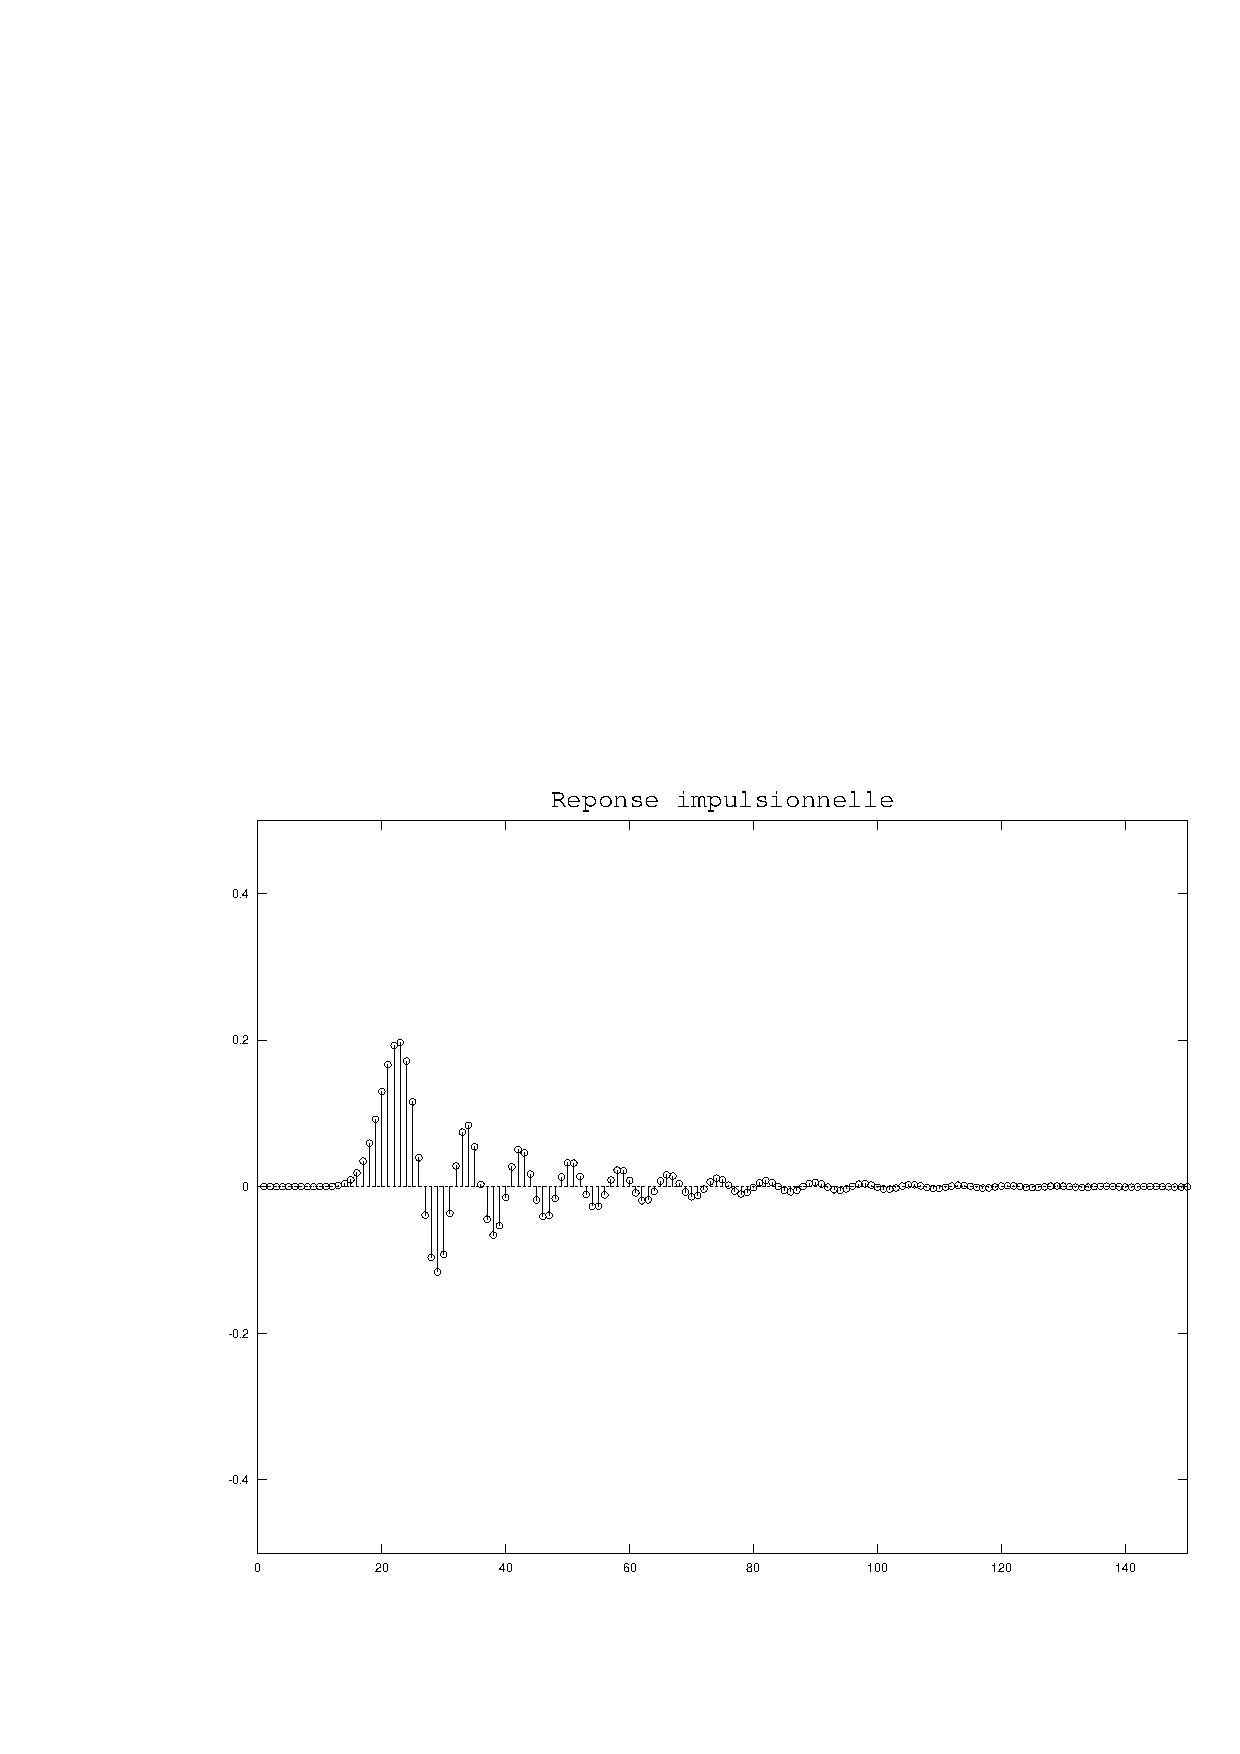
\includegraphics[width=9cm]{resEx4/repImpulsion.pdf}
\caption{Réponse impulsionnelle du filtre de Butterworth}
\end{figure}

\begin{figure}[H]
\centering
\includegraphics[width=9cm]{resEx4/ZP.pdf}
\caption{Les pôles et les zéros du filtre de Butterworth}
\end{figure}

\begin{figure}[H]
\centering
\includegraphics[width=9cm]{resEx4/fctTransfert.pdf}
\caption{Fonction de transfert du filtre de Butterworth}
\end{figure}

Le signal composé de deux sinusoïdes, une de fréquence 800 Hz et l'autre de fréquence 1.4kHz toutes deux échantillonnées à 8 kHz nous donne le signal suivant : 

\begin{figure}[H]
\centering
\includegraphics[width=9cm]{resEx4/2sin.pdf}
\caption{Signal formé de deux sinusoïdes}
\end{figure}

Le spectre de ce signal avant filtrage est représenté ci dessous:

\begin{figure}[H]
\centering
\includegraphics[width=9cm]{resEx4/spectreEntre.pdf}
\caption{Spectre d'entré}
\end{figure}

Une fois que nous lui avons appliqué le filtre nous obtenons:

\begin{figure}[H]
\centering
\includegraphics[width=9cm]{resEx4/spectreSortie.pdf}
\caption{Spectre de sortie}
\end{figure}

\part{Exercice 5}
Nous créons une fonction sinus avec les caractéristiques suivantes:\\
\begin{itemize}
\item Fréquence d'échantillonnage : 10 kHz
\item Fréquence du signal : 1 kHz 
\end{itemize}


\begin{figure}[H]
\centering
\includegraphics[width=9cm]{resEx5/fig_1_sinus.pdf}
\caption{Signal Sinus : x=$sin(2*pi*fsig*t)$}
\end{figure}


Nous ajoutons un bruit gaussien avec les caractéristiques suivantes:\\
\begin{itemize}
\item Moyenne : null
\item Amplitude : 0.4
\end{itemize}

\begin{figure}[H]
\centering
\includegraphics[width=9cm]{resEx5/fig_2_sinusb.pdf}
\caption{Signal Sinus bruité : xB=$ x .+ (moy + ampl*rand(1,N))$}
\end{figure}


Creation d'un filtre passe-bande avec buttord ayant les caractéristiques suivantes:\\
\begin{itemize}
\item Propriété : Ws(1) < Wp(1) < Wp(2) < Ws(2)
\item Ondulation maximale dans la bande passante : 3 dB
\item Atténuation minimale dans la bande coupée : 40 dB
\end{itemize}


\begin{figure}[H]
\centering
\includegraphics[width=9cm]{resEx5/fig_3_passbande.pdf}
\caption{Filtre Bande Passante visualisé sur l'intervale [900,1100]}
\end{figure}


\begin{figure}[H]
\centering
\includegraphics[width=9cm]{resEx5/fig_5_sinus-b.pdf}
\caption{Application du Filtre Bande Passante}
\end{figure}


\begin{figure}[H]
\centering
\includegraphics[width=9cm]{resEx5/fig_4_fftsinusb.pdf}
\caption{Transforme de fourier du Signal Sinus bruite}
\end{figure}


En comparant la courbe de la transformation de fourier du signal bruité FIG 42 et la courbe du signal bruité filtré FIG 41, nous remarquons autour de la frequence 1KHz ( le pic de la courbe ) que le bruit discorde moins la courbe et à donc été atténué .



\part{Exercice 6}
\lstinputlisting[caption={Code source pour l'exercice 6}, label=lst:label, language=Octave]{src/ex6.m}

\part{Exercice 7}

Deux signaux sonores S1 et S2 échantillonnés à 44.1 kHz


S1 comporter que deux composantes audibles sous la forme de deux sinusoïdes de fréquences 1000 et 3000 Hz.
\\
S1=$2*sin(2*pi*1000*t) .+ 5*sin(2*pi*3000*t)$


\begin{figure}[H]
\centering
\includegraphics[width=9cm]{resEx7/s1_audible.pdf}
\caption{Spectre de S1}
\end{figure}

Le spectre de fréquence permet de voir les 2 composantes à 1kHz et à 3kHz.
\\\\\\


S2 comporte un signal inaudible à 43.5 kHz: S2=$5*sin(2*pi*43100*t)$

\begin{figure}[H]
\centering
\includegraphics[width=9cm]{resEx7/s2_inaudible.pdf}
\caption{Spectre de S2}
\end{figure}

La fréquence du signal inaudible ne respecte pas la condition de Shannon.

En effet, si on veut échantillonner sans perdre d'information un signal à spectre limité, il faut échantillonner ce signal à une fréquence au moins égale au double de la plus haute fréquence qu'il contient.



\part{Annexe}
\section{Exercice1}
tinputlisting[caption={Code source pour l'exercice 1}, label=lst:label, language=Octave]{src/ex1.m}
\section{Exercice2}
\lstinputlisting[caption={Code source pour l'exercice 2}, label=lst:label, language=Octave]{src/ex2.m}
\section{Exercice3}
\subsection{Fonction $\frac{1-z^{-1}}{2}$}
\lstinputlisting[caption={Code source pour l'exercice 3 fonction $\frac{1-z^{-1}}{2}$}, label=lst:label, language=Octave]{src/ex3-1.m}

\subsection{Fonction $\frac{1+z^{-1}}{2}$}
\lstinputlisting[caption={Code source pour l'exercice 3 fonction $\frac{1+z^{-1}}{2}$}, label=lst:label, language=Octave]{src/ex3-2.m}

\subsection{Fonction $\frac{1-z^{-2}}{2}$}
\lstinputlisting[caption={Code source pour l'exercice 3 fonction $\frac{1-z^{-2}}{2}$}, label=lst:label, language=Octave]{src/ex3-3.m}

\subsection{Fonction $\frac{2z^{-1}}{2-z^{-1}}$}
\lstinputlisting[caption={Code source pour l'exercice 3 fonction $\frac{2z^{-1}}{2-z^{-1}}$}, label=lst:label, language=Octave]{src/ex3-4.m}

\subsection{Fonction $\frac{2z^{-1}-z^{-5}}{2-z^{-1}}$}
\lstinputlisting[caption={Code source pour l'exercice 3 fonction $\frac{2z^{-1}-z^{-5}}{2-z^{-1}}$}, label=lst:label, language=Octave]{src/ex3-5.m}

\section{Exercice 4}
\lstinputlisting[caption={Code source pour l'exercice 4}, label=lst:label, language=Octave]{src/ex4.m}

\section{Exercice 5}

\section{Exercice 6}
\lstinputlisting[caption={Code source pour l'exercice 6}, label=lst:label, language=Octave]{src/ex6.m}

\section{Exercice 7}

\section{Fonction échelon}
\lstinputlisting[caption={Fonction pour créer un echelon}, label=lst:label, language=Octave]{src/echelon.m}

\end{document} % fin du document
%EOF

